\documentclass[10pt,a4paper]{article}

\usepackage{appendix}
\usepackage{graphicx}
\usepackage{biblatex}
\usepackage{parskip}
\usepackage{listings}
\usepackage{caption}
\usepackage{subcaption}
\usepackage{amsmath}
\usepackage{listings}
\usepackage{xcolor}
\usepackage[most]{tcolorbox}

%%%%%%%%%%%%%%%%%%%%%%%%%%%%%%%%%%%%%%%%%%%%%%%%%%%%%%%%%%%%%%%%%%%%%%%%%%%%%%%%%%%%%%%%%%%%%%%%%%%%%%%%%%
\definecolor{codegreen}{rgb}{0,0.6,0}
\definecolor{codegray}{rgb}{0.5,0.5,0.5}
\definecolor{codepurple}{rgb}{0.58,0,0.82}
\definecolor{backcolour}{rgb}{1,1,1}

\lstdefinestyle{mystyle}
{
  backgroundcolor=\color{backcolour},  
  commentstyle=\color{codegreen},
  keywordstyle=\color{magenta},
  numberstyle=\tiny\color{codegray},
  stringstyle=\color{codepurple},
  basicstyle=\ttfamily\footnotesize,
  breakatwhitespace=false,     
  breaklines=true,         
  captionpos=b,          
  keepspaces=true,         
  numbers=left,          
  numbersep=5pt,         
  showspaces=false,        
  showstringspaces=false,
  showtabs=false,         
  tabsize=2
}

\lstset{style=mystyle}
%%%%%%%%%%%%%%%%%%%%%%%%%%%%%%%%%%%%%%%%%%%%%%%%%%%%%%%%%%%%%%%%%%%%%%%%%%%%%%%%%%%%%%%%%%%%%%%%%%%%%%%%%%

\lstset{basicstyle=\ttfamily, breaklines = true, tabsize=2}
\graphicspath{ {./Images/} }
\setlength{\parskip}{1em}
\begin{document}
%%%%%%%%%%%%%%%%%%%%%%%%%%%%%%%%%%%%%%%%%%%%%%%%%%%%%%%%%%%%%%%%%%%%%%%%%%%%%%%%%%%%%%%%%%%%%%%%%%%%%%%%%%

\begin{titlepage}
	\centering
	{\scshape\LARGE Imperial College London \par}
	\vspace{1cm}
    {\scshape\Large Computer Architecture: Year 2\par}
    \vspace{1.5cm}
	{\huge\bfseries 5: Memory \par}
	\vspace{2cm}
	{\Large\ Xin Wang }
	\vfill
	{\large \today\par}
\end{titlepage}

%%%%%%%%%%%%%%%%%%%%%%%%%%%%%%%%%%%%%%%%%%%%%%%%%%%%%%%%%%%%%%%%%%%%%%%%%%%%%%%%%%%%%%%%%%%%%%%%%%%%%%%%%%

\tableofcontents
\pagebreak

%%%%%%%%%%%%%%%%%%%%%%%%%%%%%%%%%%%%%%%%%%%%%%%%%%%%%%%%%%%%%%%%%%%%%%%%%%%%%%%%%%%%%%%%%%%%%%%%%%%%%%%%%%
\section{Introduction}

From the earliest days of computing, programmers have wanted unlimited amounts of fast memory. This
is practically unachievable but programmers can create an illusion of it. Before looking at creating
the illusion, first consider a simple analogy that illustrates the key principles and mechanisms.

Suppose you were a student writing a term paper on important historical developments in computer
hardware. 
\begin{itemize}
    \item You are sitting at a desk in a library with a collection of books that you have pulled from the shelves and are examining. 
    \item You find that several of the important computers that you need to write about are described in the books you have, but there is nothing about the EDSAC.
    \item Therefore, you go back to the shelves and look for an additional book. You find a book on early British computers that covers the EDSAC.
    \item Once a good selection of books is on the desk, there is a good probability that many of the topics you need can be found in them, and you may spend most of your time just using the books on the desk without going back to the shelves.
    \item Having several books on the desk in front of you saves time compared to having only one book there and constantly having to go back to the shelves to return it and take out another.
    \item The same principle allows us to create the illusion of a large memory that we can access as fast as a very small memory.
\end{itemize}

This \textbf{principle of locality} underlies both the way in which you did your work in the library
and the way that programs operate. 

\begin{tcolorbox}[breakable,colback=white]
\textbf{Principle of locality}: Programs access a relatively small portion of their address space at
any instant of time, just as you accessed a very small portion of the library’s collection.
\\
\\
\textbf{Temporal locality} (locality in time): The principle stating that if a data location is
referenced then it will tend to be referenced again soon.
\\
\\
\textbf{Spatial  locality} (locality  in  space): The locality principle stating that if a data location is
referenced, data locations with nearby addresses will tend to be referenced soon.
\end{tcolorbox}

\pagebreak

\begin{figure} [h!]
    \centering
    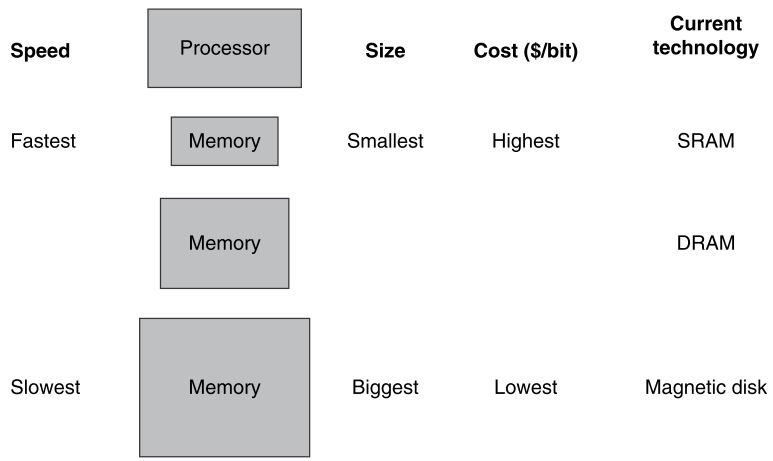
\includegraphics[scale=0.6]{Mem.JPG}
    \caption{The basic structure of a memory hierarchy.}
\end{figure}

Just as accesses to books on the desk naturally exhibit locality, locality in programs arises from
simple and natural program structures. 
\begin{itemize}
    \item Most programs contain loops, so instructions and data are likely to be accessed repeatedly i.e. high \textbf{temporal locality}.
    \item Since instructions are normally accessed sequentially, programs also show high \textbf{spatial locality}.
\end{itemize} 

The benefit of principle of locality is used by implementing the memory of a computer as a memory
hierarchy. A memory hierarchy consists of multiple levels of memory with different speeds and sizes.
The faster memories are more expensive per bit than the slower memories and thus are smaller.

\begin{tcolorbox}[breakable,colback=white]
\textbf{Memory hierarchy}: A structure that uses multiple levels of memories; as the distance from
the processor increases, the size of the memories and the access time both increase.
\end{tcolorbox}

The faster memory is close to the processor and the slower, less expensive memory is below it. The
goal is:
\begin{itemize}
    \item Present the user with as much memory as is available in the cheapest technology
    \item Providing access at the speed offered by the fastest memory
\end{itemize}

\pagebreak

\begin{figure} [h!]
    \centering
    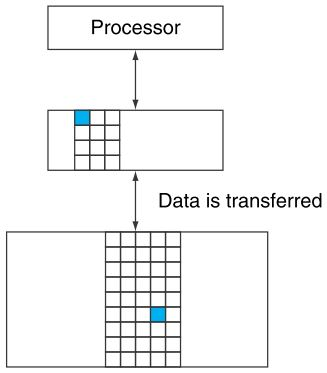
\includegraphics[scale=0.7]{Hier.JPG}
\end{figure}

A memory hierarchy can consist of multiple levels, but data is copied between only two adjacent
levels at a time, so focus is on just two levels: Upper level and Lower level. The upper level is the one closer to the processor. This is smaller and faster than the lower level, since the upper level uses technology that is more expensive

The minimum unit of information that can be either present or not present in hierarchy is called a block or a line; in the library analogy, a block of information is one book.

\begin{tcolorbox}[breakable,colback=white]
\textbf{Block (or line)}: The minimum unit of information that can be either present or not present in a cache.
\end{tcolorbox}

If the data requested by the processor appears in some block in the upper level, this is called a
\textbf{hit}. If the data is not found in the upper level, the request is a \textbf{miss}. The lower level in the hierarchy is then accessed to retrieve the block containing the 
requested data. 

The \textbf{hit rate} or \textbf{hit ratio} is the fraction of memory accesses found in the upper
level; it is often used as a measure of the performance of the memory hierarchy. The \textbf{miss
rate} i.e. $1 - \text{hit rate}$ is the fraction of memory accesses not found in the upper level.

\begin{tcolorbox}[breakable,colback=white]
\textbf{Hit rate}:  The fraction of memory accesses found in a level of the memory hierarchy.
\\
\\
\textbf{Miss rate}: The fraction of memory accesses not found in a level of the memory hierarchy.
\end{tcolorbox}

\pagebreak

Since performance is the major reason for a memory hierarchy, the time to service hits and misses is
important.
\begin{itemize}
    \item Hit time is the time to access the upper level of the memory hierarchy, which includes
    the time needed to determine whether the access is a hit or a miss.
    \item The miss penalty is the time to replace a block in the upper level with the corresponding block from the lower level, plus the time to deliver this block to the processor.
\end{itemize}  
Because the upper level is smaller and built using faster memory parts, the hit time will be much smaller than the time to access the next level in the hierarchy, which is the major component of the miss penalty.

\begin{tcolorbox}[breakable,colback=white]
\textbf{Hit time}: The time required to access a level of the memory hierarchy, including the time needed 
to determine whether the access is a hit or a miss.
\\
\\
\textbf{Miss penalty}: The time required to fetch a block into a level of the memory hierarchy from the lower 
level. This includes the time to access the block, transmit it from one level to the other, insert it in
the level that experienced the miss, and then pass the block to the requestor.
\end{tcolorbox}

\pagebreak

%%%%%%%%%%%%%%%%%%%%%%%%%%%%%%%%%%%%%%%%%%%%%%%%%%%%%%%%%%%%%%%%%%%%%%%%%%%%%%%%%%%%%%%%%%%%%%%%%%%%%%%%%%
\section{Caching}

In the library example, the desk acted as a cache i.e. a safe place to store things that needed to
be examined. Cache is the name chosen to represent the level of the memory hierarchy between the
processor and main memory.

Consider a very simple cache in which the processor requests are \textbf{each one word} and the
blocks also consist of a \textbf{single word}. Before a request, the cache contains a collection of recent references $X_1, X_2,\dots, X_{n-1}$, and the processor requests a word $X_n$ that is not in the cache. This 
request results in a miss, and the word $X_n$ is brought from memory into the cache. 
\begin{figure} [h!]
    \centering
    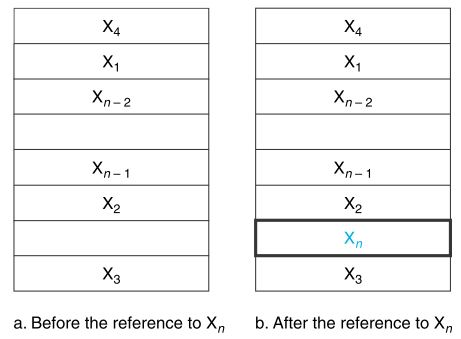
\includegraphics[scale=0.7]{Cache.JPG}
\end{figure}

The two questions that arises from this is: 
\begin{itemize}
    \item How does one know if a data item is in the cache?
    \item If it is, how is it found?
\end{itemize} 

If each word can go in exactly one place in the cache, then it is straightforward to find the word
if it is in the cache. The simplest way to assign a location in the cache for each word in memory is
to \textbf{assign the cache location based on the address of the word in memory} i.e.
\textbf{direct-mapped cache}.

\begin{tcolorbox}[breakable,colback=white]
\textbf{Direct-mapped cache}: A cache structure in which each memory location is mapped to exactly
one location in the cache.
\end{tcolorbox}

The most common mapping that almost all direct-mapped caches use to find a block:
\begin{align*}
    (\text{Block address}) \; \text{modulo} \; (\text{Number of blocks in the cache})
\end{align*}

For example, an 8-block cache uses the three lowest bits of the block address because $8 = 2^3$.

\pagebreak

\begin{figure} [h!]
    \centering
    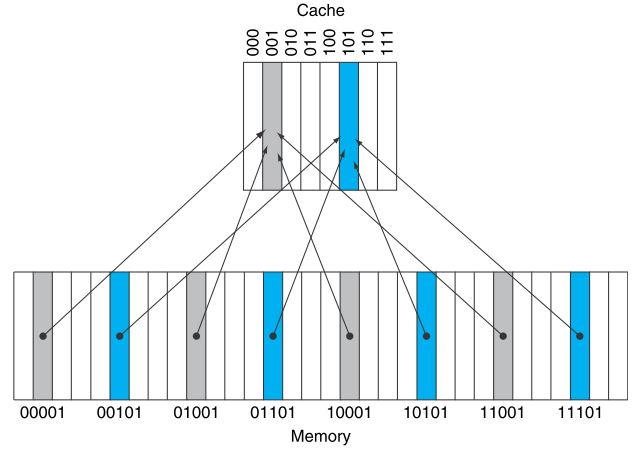
\includegraphics[scale=0.7]{Mod.JPG}
\end{figure}

With this form mapping, there arises a question: \textit{Because each cache location can contain the
contents of a number of different memory locations, how do we know whether the data in the cache
corresponds to a requested word?} This problem is solved by using \textbf{tags}.

\begin{tcolorbox}[breakable,colback=white]
\textbf{Tags}:  A field in a table used for a memory hierarchy that contains the address information required 
to identify whether the associated block in the hierarchy corresponds to a requested word.
\end{tcolorbox}

The tag needs only to contain the upper portion of the address, the bits that are not used as an index in
the cache. For example, in Figure 5.8, only the upper 2 of the 5 address bits is in the tag, since
the lower 3-bit are used in the selecting the cache block. 

A way is needed to recognize that a cache block does not have valid information. For example, when a
processor starts up, the cache does not have good data, and the tag fields will be meaningless even
if the value matches.  The most common method is to add a valid bit to indicate whether an entry
contains a valid address. If the bit is not set, there cannot be a match for this block.

\begin{tcolorbox}[breakable,colback=white]
\textbf{Valid bit}:  A field in the tables of a memory hierarchy that indicates that the associated block 
in the hierarchy contains valid data.
\end{tcolorbox}

\pagebreak

%%%%%%%%%%%%%%%%%%%%%%%%%%%%%%%%%%%%%%%%%%%%%%%%%%%%%%%%%%%%%%%%%%%%%%%%%%%%%%%%%%%%%%%%%%%%%%%%%%%%%%%%%%
\subsection{Reading a cache}

The behaviour of a recently referenced words replacing less recently referenced words, allows a 
cache to take advantage of temporal locality.

Recall that it is already known how to look in the cache for each possible address i.e. the low-order bits 
of an address can be used to find the unique cache entry to which the address could map.

\begin{figure} [h!]
    \centering
    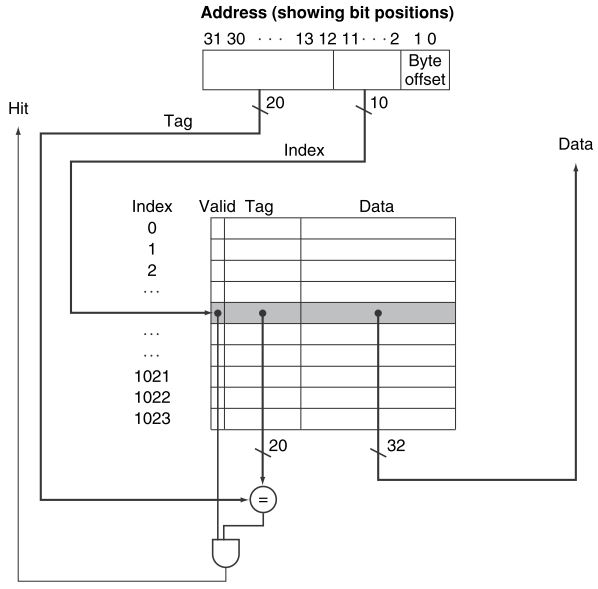
\includegraphics[scale=0.7]{Cir.JPG}
\end{figure}

The above diagram shows how a referenced address is divided into:
\begin{itemize}
    \item \textbf{Tag field}: Used to compare with the value of the tag field of the 
    cache.

    \item \textbf{Cache index}: Used to select the block
\end{itemize}

Because the index field is used as an address to reference the cache, and because an $n$-bit field
has $2^n$  values, the total number of entries in a direct-mapped cache must be a power of 2. In the
MIPS architecture, recall that words are aligned to multiples of four bytes, the least significant two
bits of every address specifying a byte within a word. Hence, the least significant two bits can be
ignored when selecting a word in the block.

The total number of bits needed for a cache is a function of the \textbf{cache size} and the
\textbf{address size}, because the cache includes both the storage for the data and the tags.

\pagebreak

The size of the block above was one word, but normally it is several. For the following situation:
\begin{itemize}
    \item 32-bit addresses
    \item A direct-mapped cache
    \item The cache size is $2^n$ blocks, so $n$ bits are used for the index
    \item The block size is $2^m$ words ($2^{m+2}$ bytes), so $m$ bits are used for the word within 
    the block, and two bits are used for the byte part of the address
\end{itemize}

Size of the tag field: $$32 - (n  + m + 2)$$

Total number of bits in a direct-mapped cache: $$2^n \times (\text{block size} + \text{tag size} + \text{valid field size})$$

\textbf{Example 1}: How many total bits are required for a direct-mapped cache with 16 KiB of 
data and 4-word blocks, assuming a 32-bit address?
\begin{itemize}
    \item 16 KiB is 4096 ($2^{12}$) words
    \item With a block size of 4 words ($2^2$), there are 1024 ($2^{10}$) blocks 
    \item  Each block has $4 \times 32$ or $128$ bits of data plus a  tag, which is $32 - 10 - 2 -
    2$ bits, plus a valid bit. 
    \begin{align*}
        2^{10} \times (4 \times 32 + (32 - 10 - 2 - 2) + 1) = 2^{10}  \times 147 = 147 \text{Kibibits}
    \end{align*}
\end{itemize}

Larger blocks exploit spatial locality to lower miss rates, increasing the block size usually
decreases the miss rate. The miss rate will eventually go up if the block size becomes a significant
fraction of the cache size, because the number of blocks that can be held in the cache will become
small, and there will be a great deal of competition for those blocks. As a result, a block will be
replaced in the cache before its words are accessed. 

A more serious problem associated with just increasing the block size is that the cost of a miss
increases. The miss penalty is determined by the time required to fetch the block from the next
lower level of the hierarchy and load it into the cache. The result is that the increase in the
miss penalty overwhelms the decrease in the miss rate for blocks that are too large, and cache performance 
thus decreases.
\begin{figure} [h!]
    \centering
    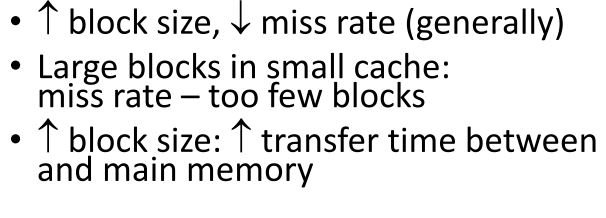
\includegraphics[scale=0.4]{Big.JPG}
\end{figure}

\pagebreak

%%%%%%%%%%%%%%%%%%%%%%%%%%%%%%%%%%%%%%%%%%%%%%%%%%%%%%%%%%%%%%%%%%%%%%%%%%%%%%%%%%%%%%%%%%%%%%%%%%%%%%%%%%
\subsubsection{Handling misses}

\begin{tcolorbox}[breakable,colback=white]
\textbf{Cache miss}: A request for data from the cache that cannot be filled because the data is not
present in the cache.
\end{tcolorbox}

The control unit must detect a miss and process the miss by fetching the requested data from 
memory. If the cache reports a hit, the computer continues using the data as if nothing happened.

The processing of a cache miss creates a pipeline stall instead of an interrupt. The pipeline stall
would require saving the state of all registers. For a cache miss, the entire processor is stalled,
essentially freezing the contents of the temporary and programmer-visible registers while the memory
is accessed.

Steps to be taken on an instruction cache miss:
\begin{itemize}
    \item Restore PC: Send the original PC value (current PC - 4) to the memory.
    \item Instruct main memory to perform a read and stall for the memory to complete its access.
    \item Write data received from memory to cache.
    \item Refetch instruction from restored PC.
\end{itemize}

The process is similar for a \textbf{cache miss on data read}.

%%%%%%%%%%%%%%%%%%%%%%%%%%%%%%%%%%%%%%%%%%%%%%%%%%%%%%%%%%%%%%%%%%%%%%%%%%%%%%%%%%%%%%%%%%%%%%%%%%%%%%%%%%
\subsection{Writing to a cache}

Writes are very different. The main problem: consider on a store instruction e.g. STO, data is
only written into the cache without changing the main memory content. After the write operation, the
memory content would be different from the cache content. This is the problem of \textbf{data coherency}.

In such a case, the cache and memory are said to be \textbf{inconsistent}. The simplest way to keep
the main memory and the cache consistent is always to write the data into both the memory and the
cache. This scheme is called \textbf{write-through}.

\begin{tcolorbox}[breakable,colback=white]
\textbf{Write-through}: A scheme in which writes always update both the cache and the next lower
level of the memory hierarchy, ensuring that data is always consistent between the two.
\end{tcolorbox}

\pagebreak

There are two classical approaches that highlight the weakness that need to be solved:
\begin{itemize}
    \item Write back:  Write to cache only. Complex control needed, thus adding extra bits for cache entries.
\end{itemize}

\begin{tcolorbox}[breakable,colback=white]
\textbf{Write-back}: A scheme that handles writes by updating values only to the block in the cache,
then writing the modified block to the lower level of the hierarchy when the block is replaced.
\end{tcolorbox}

\begin{itemize}
    \item Write through: Write to both cache and memory. The memory write bandwidth causes a severe bottleneck.
\end{itemize}

One solution to this problem is to use a write buffer between cache and memory.

\begin{tcolorbox}[breakable,colback=white]
\textbf{Write buffer}: A FIFO queue that holds data while the data is waiting to be written to memory.
\end{tcolorbox}

The new write process:
\begin{itemize}
    \item Processor writes into write buffer and cache. After writing the data into the 
    cache and write buffer, the processor continues execution sequence.
    \item Memory controller writes the content of the write buffer into memory.
    
    When a write to main memory completes, the entry in the write buffer is freed. If the write buffer 
    is full when the processor reaches a write, the processor must stall until there is an empty
    position in the write buffer.
\end{itemize}

If the rate at which the memory can complete writes is less than the rate at which the processor is generating writes, no amount of buffering can help, because writes are being generated faster than the 
memory system can accept them. This is known as \textbf{buffer saturation}.
\begin{align*}
    \text{Store frequency} << \frac{1}{\text{Memory write time}}
\end{align*}

Buffer saturation is caused when:
\begin{itemize}
    \item CPU cycle time too short w.r.t. memory speed
    \item Too many store instructions in a row
\end{itemize}

And the solutions to buffer saturation:
\begin{itemize}
    \item Use a write-back cache
    \item Install a second-level (L2) cache
    \item Store compression
\end{itemize}

\pagebreak

%%%%%%%%%%%%%%%%%%%%%%%%%%%%%%%%%%%%%%%%%%%%%%%%%%%%%%%%%%%%%%%%%%%%%%%%%%%%%%%%%%%%%%%%%%%%%%%%%%%%%%%%%%
\section{Cache Performance}

There are two different techniques for improving cache performance:
\begin{itemize}
    \item Reducing the miss rate by reducing the probability that two different memory blocks will contend for the same cache location. 
    \item Reduces the miss penalty by adding an additional level to the hierarchy i.e. \textbf{multi-level caching}.
\end{itemize}

CPU time can be divided into the clock cycles that the CPU spends executing the program and the
clock cycles that the CPU spends waiting for the memory system.
\begin{align*}
    \text{CPU time} = (\text{(Execution cycles}+\text{Memory-stall cycles}) \times \text{Cycle time}
\end{align*}

Memory-stall cycles can be defined as the sum of the stall cycles coming from reads plus those
coming from writes:
\begin{align*}
    \text{Memory-stall clock cycles}=(\text{Read-stall cycles }+\text{ Write-stall cycles})
\end{align*}

The read-stall cycles can be defined in terms of the number of read accesses per program, the miss penalty in clock cycles for a read, and the read miss rate:
\begin{figure} [h!]
    \centering
    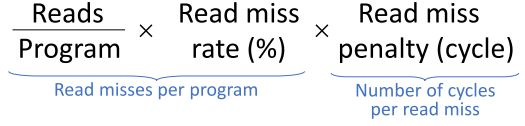
\includegraphics[scale=0.5]{eq.JPG}
\end{figure}

For a write-through scheme, there are two sources of stalls:
\begin{itemize}
    \item Write misses, which usually require that we fetch the block before continuing the write.
    \item Write buffer stalls, which occur when the write buffer is full when a write occurs. 
\end{itemize}  
\begin{figure} [h!]
    \centering
    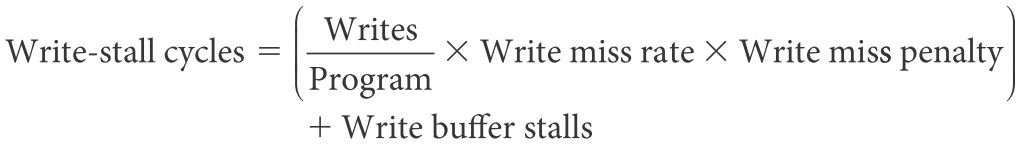
\includegraphics[scale=0.5]{eq1.JPG}
\end{figure}

%%%%%%%%%%%%%%%%%%%%%%%%%%%%%%%%%%%%%%%%%%%%%%%%%%%%%%%%%%%%%%%%%%%%%%%%%%%%%%%%%%%%%%%%%%%%%%%%%%%%%%%%%%
\pagebreak

\subsection{Effect on CPU}

\begin{figure} [h!]
    \centering
    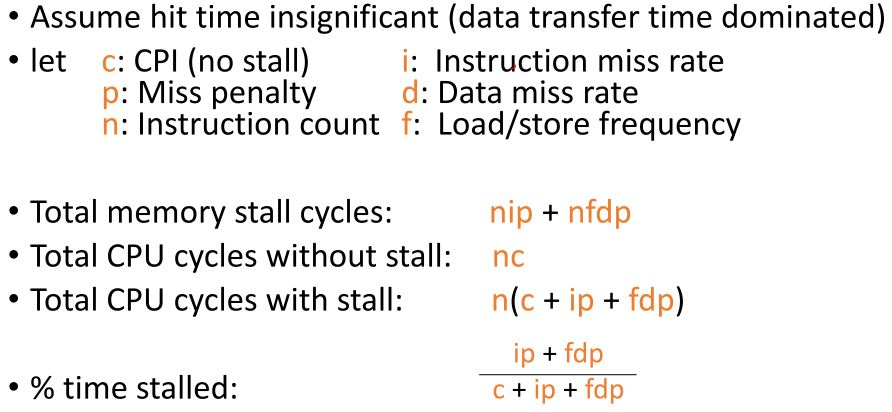
\includegraphics[scale=0.5]{A.JPG}
\end{figure}

%%%%%%%%%%%%%%%%%%%%%%%%%%%%%%%%%%%%%%%%%%%%%%%%%%%%%%%%%%%%%%%%%%%%%%%%%%%%%%%%%%%%%%%%%%%%%%%%%%%%%%%%%%
\subsection{Average Memory Access Time}

\begin{figure} [h!]
    \centering
    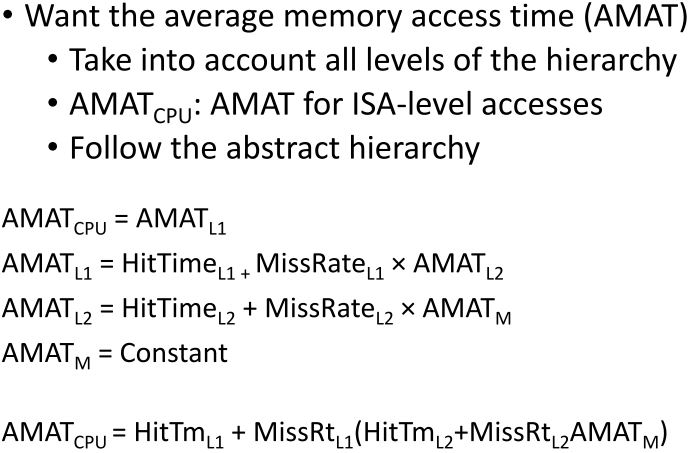
\includegraphics[scale=0.5]{B.JPG}
\end{figure}

\pagebreak
%%%%%%%%%%%%%%%%%%%%%%%%%%%%%%%%%%%%%%%%%%%%%%%%%%%%%%%%%%%%%%%%%%%%%%%%%%%%%%%%%%%%%%%%%%%%%%%%%%%%%%%%%%
\section{Associative cache}

So far, only a simple placement scheme is used: A block can go in exactly one place in the cache. As mentioned earlier, it is called direct mapped because there is a direct mapping from any block address in memory to a single location in the upper level of the hierarchy. However, there is actually a 
whole range of schemes for placing blocks with direct mapping on one end of the extreme.

At the other extreme is a scheme called \textbf{fully associative}, because a block in memory may be
associated with any entry in the cache. To find a given block in a fully associative cache, all the
entries in the cache must be searched because a block can be placed in any one.

\begin{tcolorbox}[breakable,colback=white]
\textbf{Fully associative}: A cache structure in which a block can be placed in any location in the
cache.
\\
\\
\textbf{Set-associative cache}: A cache that has a fixed number of locations (at least two) where each 
block can be placed.
\end{tcolorbox}

To make the search practical, it is done in parallel with a comparator associated with each cache
entry. These comparators significantly increase the hardware cost, effectively making fully
associative placement practical only for caches with small numbers of blocks.

The differences between direct mapped and fully associative:
\begin{itemize}
    \item Direct mapped: Simple, fast accesses, high miss rates
    \item Fully associative: Low miss rates, costly, slow (need to search everywhere)
\end{itemize}

\begin{figure} [h!]
    \centering
    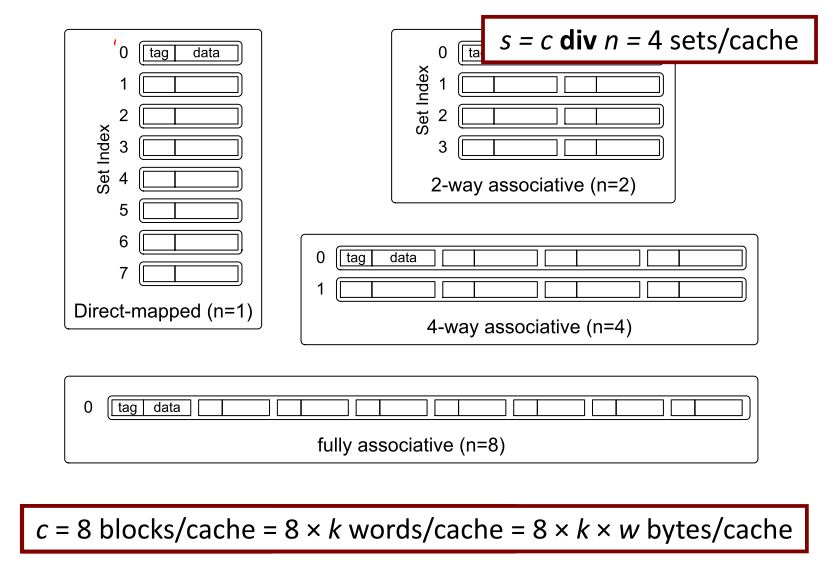
\includegraphics[scale=0.6]{cache1.JPG}
\end{figure}













%%%%%%%%%%%%%%%%%%%%%%%%%%%%%%%%%%%%%%%%%%%%%%%%%%%%%%%%%%%%%%%%%%%%%%%%%%%%%%%%%%%%%%%%%%%%%%%%%%%%%%%%%%
\end{document}